
\chapter{Rag Doll}

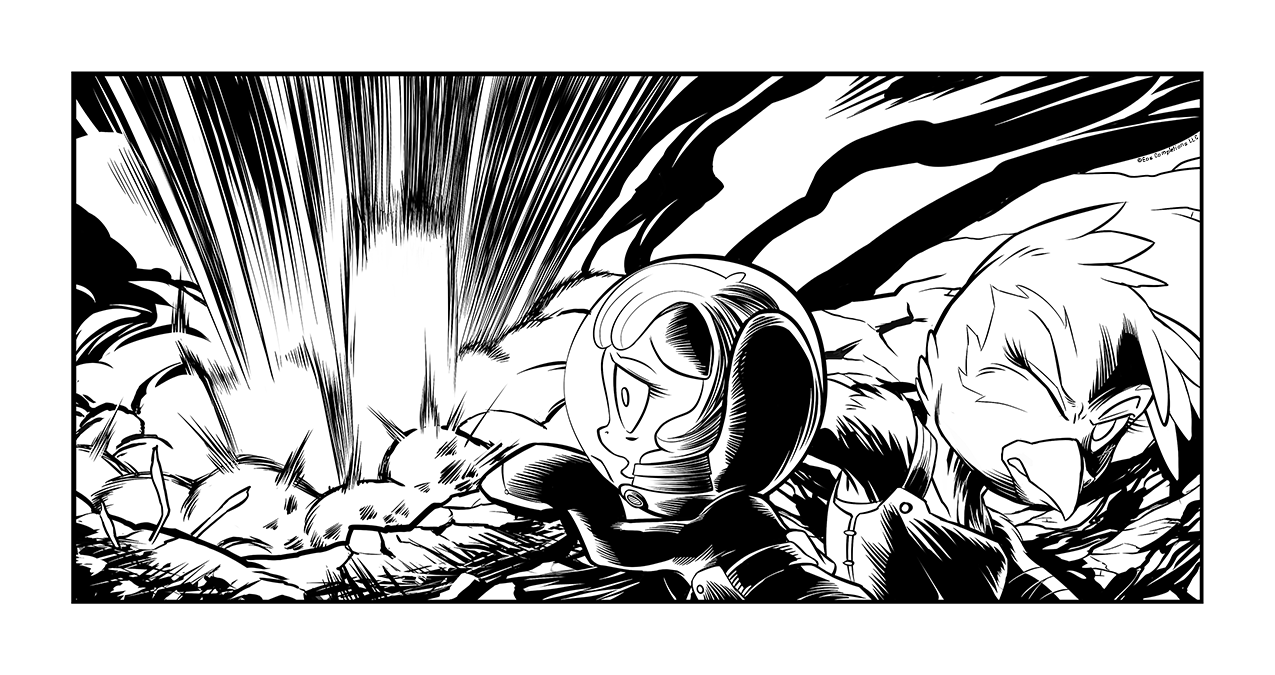
\includegraphics[width=0.9\linewidth]{image14.png}

\begin{intro}
Into each life some rain must fall\dots
\end{intro}


\englishdaytimeplace{11}{22:30 P.M.}{Low orbit, $\approx \SI{1800}{km}$ above Equestria}

High above the planet floated Ponymedes I, a giant of plastic and super light alloys that had a body shaped like a large sunflower and long solar panels that formed its petals. There were words and signs painted across the satellite that warned against a multitude of dangers, such as fire or falling rocks, but the only one that held some meaning for an observer was the Solaris logo, with its male alicorn and the company motto ``Try the alternative'' encircling the image.

Attached to the satellite's large round body there were four barrels, easily longer than a couple train cars. The weapons were composed of two linear metal rails held together by many rings, placed only a few centimeters apart from each other. It functioned as a weapon that use a sequence of strong, magnetic pulses, and a potent electric thrust to propel a metallic body at unpony speed against very distant targets. In other words, it was a deadly weapon, and Ponymedes I was armed with four of those little toys.

But at Solaris, nopony left a work half-baked. How could a single satellite always be ready for action? They needed a network of satellites, a complete shield ready to defend Equestria or whomever made a better offer for that little jewel. Ponymedes had eleven siblings, able to change their distance from the planet and move around in orbit to operate in groups. Now the whole family had been reunited, and each of the twelve brothers had their guidance lasers pointed at their own designated target.

{\mt ``\dots Eight\dots seven\dots six\dots''}

As one, the four barrels began to discharge sparks of blue electricity from between each ring and all along the metal rails as the the countdown steadily ticked away. A metallic bar coated in ceramics, more or less one and a half meters long, and shaped like a pointy stick, was placed into the barrel by an automated loading system and immediately enveloped by a blue halo.

{\mt ``\dots Five\dots four\dots three\dots''}

Behind the satellite, four hatches opened to reveal the exhaust vents for the recoil compensation system, a dim red light appeared inside each of them, glowing like lava within the belly of a volcano. All four barrels were now completely blue, powered by the electricity running from ring to ring. They resembled four bright lances, ready to unleash their fury against a doomed opponent.

{\mt ``\dots Two\dots one\dots''}

{\mt Fire.}



\horizonline

\englishdaytimeplace{11}{22:30 P.M.}{Ivory Tower, Big 52 SC Branch}

{\mt ``Attack commenced. Estimated time of arrival for the first salvo: seven minutes.''}

Half of the guidance lasers disappeared, and a couple shifted kilometers away in the blink of an eye, as if something up in the heavens had gone awfully wrong. Still, five red lights continued to shine down on the building's roof, flickering once or twice, but staying on target.

``Why is everyone retreating now?'' Henrietta opened her wings, ready to grab Puppy and fly away with her.

Puppy pointed at the besieged building entrance. ``Those two aren't running away, we can ask them!'' And with these words she tried to trot towards the two perplexed paladins defending the main research building.

``I don't think so! My job is done here, and we're following the example of our fleeing friends.''

``TO ALL THE PONIES INSIDE THE BUILDING! YOU ARE BEING ATTACKED FROM THE SKY! EVACUATE THE FORT! WE CALL FOR A TRUCE! RUN FOR YOUR LIVES!'' Once again, Scold's voice thundered above the battlefield before he turned on his tail and ran, following the acolytes and the other scribes.

Finally, Henri looked up at the clouds, and her beak hung open as she saw the red lasers cutting through the darkness of the night. ``Oh, rotten eggs. If those are what it uses to aim, I don't want to see what it fires!''

{\mt ``Warning. Lost signal from Ponymedes III, V, X, XI and XII. Ponymedes IV and VII report major failures with the recoil compensation system. Ponymedes I, II, VI, VIII and IX are commencing the second barrage in ten\dots nine\dots''}

Puppy frowned. Mr. Voice had been talking for a while now, and it didn't seem like he was going to stop any time soon. Everything was becoming really confusing. Why was everypony running away? Why was Mr. Red Cape yelling so loud, and why was her helmet showing her all these blinking red lights everywhere? ``How do I make all this mess stop?''

``I don't know. I don't care! Let's get out of here!'' Henri took flight, grabbing Puppy and gaining height and speed with each stroke of her eagle wings.

Okay, new problem. Flying. Puppy had thought up a plan for the next time she had to fly, something she really, really had to do. What was that already? Oh, right, scream. ``EEEEEEP! NONONONONO!''

``Shut that trap! I'm trying to save your life!'' After her running start, Henri began to lose speed and altitude, dragged down by Puppy's weight. ``What the fuck are you carrying around now? I made you throw away a ton of junk, and you're already full of useless stuff again! Aargh! Unload the bags or we'll crash!''

{\mt ``\dots two\dots one\dots Second salvo out. Readying guns for third salvo.''}

``LEMME GO! LEMME GOOO!'' Puppy was struggling, in the middle of her personal world of things moving too fast and too far from her hooves to be comfortable with.

Henrietta tried cutting one of her saddlebags with a talon, slashing desperately at the bottom of the container, and missing it several times before finally managing to hit the moving target. ``Gotcha!''

{\mt ``Repair spell activated. Lost signal from Ponymedes I and II. Ponymedes VI, VII and XI will be ready to fire in ten\dots nine\dots''}

The hole in the bag closed almost immediately, while the inventory management spell kept everything in its place.

``Hey, that's cheating! Do you want to play rough? I'm in!'' She let go of Puppy from one side, turning her upside down. This strategy worked a little better because one of the bags wasn't closed. Puppy rapidly lost weight as she left behind a trail of odds and ends in the sky: empty bottles, roasted plushies, and a small toy cart.

``NONONO! I'm gonna pee myseeeeelf! Please stop! PLEASE!'' Puppy was completely terrorized by the situation, and being dangled in the sky like that only made things worse. She succeeded in grabbing The Rock Of Destiny as it fell from her bag, although a lot of the cool stuff she found was lost forever. Everything was going bad today, and she didn't even have time to complain, since stoopid chicken Henri was teasing her hard. ``You bully, let me go or I'm telling Mom!''

When Puppy had finally reached a bearable weight, Henri lifted Puppy onto her back, hoping that that would lessen the screams. ``All right, all right! We're done, now be quiet and I'll put you down when we pass that hill!'' Henri had no idea of what was going to rain down from the sky, but her life as a mercenary had taught her the value of cover. Actually, she wondered why nothing had happened yet, but she suspected that the longer whatever it was took to arrive, the worse it was going to be. ``We can't land here, Puppy! Try not thinking about it. Listen to some music and close your eyes!''

Puppy was barely listening, but the music idea suddenly seemed like the best idea ever. ``Music! Now, please!''

The radio came to life, while on the ground ponies ran as fast as they could. Both the Applejack's Rangers and the Steel Rangers who had decided to believe the old scribe were now running for the hills.

\rtpr{``Hello fillies and gentlecolts! Isn't it well past your bedtime? This is Lonesome Pony, and you are listening to Radio 52, the only radio that brings you news and safety, from the Ridges to Emerald Shores! Tonight we have a lot of things to talk about, so let's get to business.''}

Not music. Why was it that every time Puppy turned on the radio, the first thing she heard was the stoopid chatty pony? Puppy wanted some music! The ground was a rushing blur down below, and Mister Voice wouldn't stop chatting, and now even Lonesome Pony was giving her a lecture instead of some music? Puppy wanted to cry. In the background, the suit informed her that the surviving three satellites were continuing their attack.

\rtpr{``First things first, Things are getting messy along the South Branch. It seems that the Wild Herd is ambushing the patrols from Ironworks again, but this time they seem to be better equipped, and way more organized than in the past. Maybe they found a new leader? This could mean big, big trouble in the near future. Don't lower your guard if you are traveling south of Broccoli, or from the Memorial to Ironworks, and try avoiding the east route to Emerald Shores. Stay on the road and turn your tails as soon as you see something suspect. Better safe than sorry!''}

Henri soared through the air, easily surpassing the ponies that led the retreat. They were slow, too slow to get to a safe distance in time, but there was a good chance that even she and Puppy were condemned, so why not try running anyway? With a stroke of her wings, Henri gained speed and kept flying straight, despite the choking grip Puppy had around her neck.

\rtpr{``Now, since bad news never trots alone, we have a new change of policy from the NCA, rejoice! The NCA forces have decided that every trader is actually a raider, so they started arresting traders and confiscating the merchandise on their borders, yay! If you were planning for a trip there, you better reconsider and try heading for Salt Cube City or Tunnel Town for trading your goods, since the northern branch is now safe.''}

Henrietta landed behind the hill, panting heavily. Puppy jumped down from her back as soon as she could see solid ground and immediately stuck out her tongue at the big meanie chicken. ``Bleh! Why do you always bully me? I'm your friend!''

``Fuck off, Puppy.'' Replying with almost no breath in her lungs was quite hard for Henri, but Puppy couldn't have things her way every time. ``I'm not bullying you. Something is going to happen in that place, something bad.''

\rtpr{``And now the last news. It seems that an old merchant came back from his longest trail. He started four years ago with a cart full of garbage and a brahmin, and he's back with, well, a brahmin, a cart full of garbage, and a lot of stories! Maybe over the next day I'll tell you all about the places he visited, but it seems that those ponies in the far west are crazy! He told me about a city of lights, and great walls crossing a river, imprisoning it to produce energy. Woah, we could use something like that, couldn't we? And this ends the news. Have some good music, my little ponies!''}

Puppy cocked her head in surprise. ``Something bad? But Mom is there!'' Puppy turned towards Ivory Tower, now more than a couple kilometers away, illuminated by the dim red light of a single surviving laser beam. The clouds above the old research facility flashed with white light for a moment.

At which point the radio decided to start playing music.

\begin{music}
		Raindrops keep falling on my mane,
	
		And just like the foal whose cutie mark is not there,
	
		Nothing seems to fit there.
\end{music}

Blazing lines of white burst through the clouds. Like tiny silver darts shining in pure heat, they rained down from the heavens onto Ivory Tower. The magnetically accelerated shots crossed the cloudy sky in a split second, striking the buildings and the area nearby with such force that for a moment, Henri could have sworn that she felt the earth shudder beneath her feet.


\begin{music}
		Raindrops are falling on my mane. They keep falling---
\end{music}

First arrived the flash. A white halo rose from the impacted structure, then the walls seemed to expand for a moment, reminding Puppy of a balloon being inflated. For a short instant, everything seemed to hang in the air, as if time had stopped, leaving the building floating there, separated into its many elements. Walls, windows, doors, all like in one of those drawings that showed all the parts of a cart or a house that Mom had shown her that one time. That instant of stillness only lasted for the blink of an eye. Then everything flew away in different directions. Chunks of wall as large as trucks went flying through the sky like shreds of paper, surpassing even the moat and landing on the bridge and shacks beyond, making them crumble like a cardboard castle.

Then came the sound. The first thing Puppy heard was an acute whistle, like when you try making that weird music with grass leaves. But it didn't last for long, because immediately after it arrived the boom. Not just one big boom, but the sound of many thuds, followed by the booming thing. It was like a rapid fire concert, a thud then a boom, a thud and a boom, a thud-thud and a badaboom. Wow, catchy.

Puppy really wished that Mom could have been there to see that show. It was so fun! No wait, Mom was there. Actually, Mom was supposed to be inside that super nice white build---oh.

Her eyes widened as she lifted a hoof towards what was once Ivory tower, her expression becoming a mask of fear. ``Mom?''


\begin{music}
		So I just did me some talking with the sun,
	
		And I said I didn't like the way she got things done.
	
		She's sleeping on the job.
\end{music}

{\mt ``Warning. Ponymedes VI is out of ammunition. Signal lost from all the other satellites. Attack aborted. Area will be safe from incoming fire in fifteen minutes. Thank you for choosing Solaris Inc. as your main siege weapon system. Solaris: try the alternative.''}

Puppy stared unblinkingly at the white points of light as they continued to pierce the clouds and rain down like tiny stars on what was once her mission objective. Why didn't they stop? Wasn't that enough? They already made a lot of noise and stuff, so now it was time to stop, right? It's fun only if it lasts a bit, but then it becomes scary. Puppy held her breath, praying that every silver shard falling from the sky was the last, but they never seemed to stop. There were always others coming.

They were destroying the place where Mister Voice told her that Mom was. But wait! The arrow was still there! Yes! There was still hope! Puppy rejoiced. Nothing could stop Mom! Take that, stoopid silver rain!

\begin{music}
		Those raindrops are dropping on my mane. They keep falling---
\end{music}

Another hail of falling stars fell in the cloud of smoke and debris, this time hitting somewhere near the research center's power plant. It was easy to tell, because the thud was followed by a ball of green fire that exploded upwards towards the sky, producing a glowing mushroom cloud in the middle of the mayhem. Okay, that was new, and it was unfair.

{\mt ``Warning. Mild radiation detected. Threat level: negligible.''}

The pink arrow on the compass blinked three times and disappeared. Puppy waited for it to reappear, hoped for it to reappear, and begged for it to reappear, but the compass remained empty. The suit informed her that the mission 'Chasing Rain' had been completed.

Why were those silver things still falling even now? It was over, all over. The arrow was gone. Mom was gone! Mom\dots was gone? No, that couldn't be! Mom was\dots Mom was where the arrow said, but now, now the arrow didn't say anything! Puppy followed that arrow only because it pointed at Mom, and now there was nothing to follow! There was nothing left, just\dots just a bunch of falling stars and---and for the first time since she left Canterlot, she didn't know what to do.

Mom was gone.

\begin{music}
		But there's one thing I know.
	
		The blues they sent to meet me,
	
		Won't defeat me.
\end{music}

Puppy's right eye twitched. She stood still, eyes wide open and staring, her muzzle petrified in an expression of surprise. Henrietta put a paw on Puppy's shoulder, trying to say something in the deafening thunders of the bombardment. Whomever began that attack wanted to be double sure that nothing was left of the whole place. Even after the generator's explosion those white missiles kept arriving. These guys had ammo to waste.

``Don't worry! Your mom wasn't there! I was inside the place, she wasn't in Ivory Tower!'' Puppy didn't react. She probably didn't even hear her words, so Henri tried shaking her, but the pony didn't offer any resistance, simply moving like a rag doll, her blonde head bobbing inside the helmet.

\begin{music}
		It won't be long till happiness steps up to greet me.
\end{music}

``Oh, c'mon, Puppy! You have been through things way worse than this! Hey, I'm talking to you!'' Henrietta poked Puppy again, making her head bob a little more. ``What the fuck? Hey, wake up!'' Still no reaction.

``We have to get away from here. That last explosion spread radiation everywhere!'' She sighed in frustration. ``Why me? I just accepted a simple job. Why is it that every fucking time I try something it goes fucking south? No wait, I don't want to know!'' Henri put Puppy on her back and started walking away, trying to catch up with the rangers.

``Whatever, those fanatics still owe me half my pay. Let's go, Puppy.'' Henri slowed her walk, feeling that something was missing. ``I can't stand you like this. Say something, please!'' Still nothing.

``Okay, you want it the hard way? Here we go!'' Henrietta waved Puppy's hoof around in the air and tried to imitate her friend's usually enthusiastic voice. ``Yush! Let's go, pretty bully chicken!''

By now the attack had begun to slow down, with only a couple of lights raining down each minute, but even those few bolts were enough to make the ground tremble.

``Great, now I'm talking with a giant puppet. This will help for sure\dots''



\horizonline

\englishdaytimeplace{12}{4:30 A.M.}{Steel Ranger's Outpost, Big 52 SC Branch}

A group of rangers, scribes, and acolytes were building an impromptu encampment next to a hillside. They were moving crates and military bags out from a reinforced blast door that was built into the natural mound.

The little bunker had been used as a monitoring station during the war, and then as an observation post by the rangers for more than a century. It was built inside a hill with a couple of raised scout platforms on top. The whole complex was a little cramped, and couldn't fit more than eight or nine ponies inside, but it was better than nothing, and the rangers had kept some supplies and spare equipment inside in case of an emergency.

``Look, things didn't go exactly as planned, so I can't spare another single cap right now.'' Cold Shower hadn't even bothered to take off her helmet before speaking with Henrietta.

She cocked her head, upset. ``But I did what you asked me to do! I disabled the generators and all their damn internal security system! I don't care if the whole place got showered with falling stars! I want my caps!''

``You could always go back into the crater and take them for yourself, we won't argue with that. Now if you'll excuse me, I have a camp to organize, decisions to make, and prisoners to manage.'' Cold Shower began to trot away from Henri.

Henrietta took Puppy's hoof, pointing it toward Cold, and spoke with a childish voice. ``You meanie pony! Why are you cheating? Stop being a bad smart robowhatever and play by the rules!''

Cold Shower froze on the spot, turning her head toward Henri, who was moving the foal like a rag doll. ``You are creepy as hell, do you know that?''

``Don't use your smarts with me! I'm not stoopid! Now behave and pay my friend!'' With a poke to the helmet, Henri made Puppy's head turn a little in her direction. This made Cold step back, shivering.

``Stop that! Listen, I'm sorry for your friend, but we have our own problems!'' Shower hesitated. She wasn't sure of what freaked her out the most: seeing the once lively filly now reduced to a veggie, or the young griffon girl using her as a money begging puppet.

Henri crossed Puppy's hooves and made her head turn away. ``I don't want to be your friend nevermore!''

``Okay, okay I give up! Listen, now we have to work out what to do with the rangers that decided to surrender. After that I'll send you to Scribe Scold, and he'll see what can be done for Puppetsmiles, ah, I mean Puppysmiles. When that's done, I'll see if I can put something together to pay you, but don't expect very much.''

Puppetsmiles raised a hoof. ``Yay~''

``And stop that puppet thing! It's creepy!'' She trotted away without waiting for another reply from Henri.

Henri stood for a moment, smiling satisfied, then walked around the hill, and as soon as the camp was out of sight, she hugged Puppy with all her strength. ``Don't worry, we will fix everything, just\dots just don't go away, please\dots''

She sat on the ground and kept talking, still hugging Puppetsmiles. ``I know I've been a bad friend, but I never meant to. It was all a joke! Have you the slightest idea of how hard the life of a mercenary is? No, you don't, you\dots You're just an immortal shade playing around and making everything seem easy and, and I envied you. I also hated you because you weren't sad, even though you were alone. I hate being alone\dots''

Scribe Scold came around the corner at that very moment, calling for Henri. ``Hey, Miss Firebright! Paladin Shower wants to talk with you in the bunker.'' Scold stopped where he was, waiting for a reply.

Henri yelped in surprise and tried desperately to hide Puppetsmiles behind her back. ``Call! Call next time!''

``Yes, sure.'' He nodded.

Her expression was one of panic and concern. ``Did you see anything?''

``No girl, I didn't see that you were hugging your friend and crying.''

Henri seemed to relax. ``Good!'' She walked toward Scold and poked him in a shoulder. ``Keep an eye on the dead weight there while I'm away.'' She paused for a moment, looking straight into the old scribe's eyes. She lost the battle almost immediately. ``Please\dots''

``No problem, I was actually looking for her on my own. Take your time.'' Scold waited for Henrietta to nod and walk away, then he trotted toward Puppy, who was sitting and staring off into the distance, still lost in some Celestia-knows-what place in her head.

``So, here we are, me and you again. I have a suspicion, and I need to take a look in your bags. Care if I do? No? Thanks.'' He didn't smile, he simply opened the suit's saddlebags and started browsing through Puppy's inventory. ``After all, you went through my stuff, so I don't see why I shouldn't return the favor. Let's see what we have here.''

\emph{A broken toy\dots colored glass\dots light bulb\dots bottle caps\dots the other half of my glasses\dots }---SQUELCH---\emph{squelch\dots squelch?}

He pulled his hoof out of the bag only to see it covered in a stinky green goo. ``For Luna's sake, what is this stench?'' Scold put on a glove and carefully took out whatever it was that had produced all that slime. ``A dead parador? Why would a foal want to keep a rotting dead parador in her bag!?''

\emph{Wait\dots A dead parador cub\dots for a little undead foal. It's---is this her pet? All right, this has ruined my day.}

Scold put the dead critter back inside the bag and went to check the other that was almost empty. Why had she put all that stuff in one bag and left the other empty? 

After a quick check of the second saddlebag, Scold found what he was looking for in the form of a target designator. Uttering a short whistle, the scribe took it in his hooves and studied the model.

``And here we have the winner. Solaris, that makes so much sense.'' He snickered, reading the weapons data on his pipbuck. ``Sentenza, meaning judgment. How appropriate.''

Looking in the distance, more or less in the same direction Puppy was turned, Scold sat beside her and continued. ``I am in your debt, little soul. If that attack wasn't interrupted, many young ponies would have died. When those lights from the sky derailed the battle, you saved lives on both sides.''

He patted Puppysmiles on her helmet. ``This battle is ridiculous. Brothers fighting brothers, and elders that care more for their own power than the good of those that surround them. Once I was told that a chief that deserves respect is a chief that gives respect to his subordinates. Our elder was\dots different, and stubborn. He would have let all of his followers die simply to defend his beliefs, not even caring if they shared those beliefs or not.''

Patting Puppy again, this time on her back, Scold sighed. ``I guess that I'll keep this little secret for myself, and Sentenza. And I'll forgive you for destroying, well, everything I possessed and cared for.'' He paused, a slight smile on his lips. ``Except for the most valuable thing I ever had: my students.'' He sighed again as his body told him he was old and tired, but somehow he was also a happy pony. Scold didn't remember the last time he felt like this, but it must have been very long ago. ``Oh well, the Big 52 gives, the Big 52 takes. And I'll give you something in return for your toy.''

``Here, be her friend, but don't dye her mane, deal?'' Scold put the Lyra doll inside Puppy's saddlebags. ``Looking at you, I wish I had a grandchild, but my son---no, I'd better not talk about that.''

He stood and trotted away, leaving Puppy to sit by herself on the hillside.

``Oh, one last thing. There is a town named Broccoli south of here, but before getting a name from what they farm, the town was called Rainy Camp, and its assembly hall is still named Rainy Days. I'm not sure if this will help you, but I don't believe in luck, so\dots You should check for yourself.''

With these last words, the pony disappeared behind the hillside.

{\mt ``Journal updated. New primary quest: Southern Storm. Broccoli Town Hall set as new primary objective. Broccoli Town Hall marked on the compass.''}

A pink arrow appeared and began to blink.



\horizonline

\englishdaytimeplace{12}{5:00 A.M.}{Steel Ranger's Outpost, Big 52 SC Branch}

Cold Shower greeted Henrietta with a nod as she entered the bunker. ``I hope my summon wasn't too hasty, but I could have a solution for both your payment and a trouble of mine.''

Henrietta took her time to look inside the room before replying to the paladin's words. The bunker central hall consisted of a large room with a low ceiling supported by a forest of pillars. There were shelves lined up against the walls, and low metal tables in the middle of the room, but instead of chairs the ponies used metal boxes that doubled as small cabinets. Henri noticed that there were no couches in this room, but there was a staircase going up, probably to the observation posts, and a couple of metal doors closed with some sort of computerized lock.

In the room there were seven ponies, two of them wore the typical power armor of the rangers, but, without their helmets, Henri was easily able to recognize them as Paladin Shower and Paladin Gauss. The other five ponies were all new faces for her. They were in chains and showed varying degrees of shame, fear or anger on their faces. Just looking at those muzzles made her aware that whatever the paladin was going to offer wouldn't be good news. ``I want double.''

Cold Shower ignored her and carried on speaking as soon as she was sure of having the mercenary's attention. ``These are Steel Rangers still faithful to the elders. They decided to capitulate instead of fighting, since the base is irremediably lost, but they won't join our ranks. They need an escort to Tunnel Town, across the desert, so a good hired gun that doubles as air recon would be perfect.''

Henrietta cocked her head. ``What am I, a foalsitter? I have my agenda, and you still owe me a load of caps!''

``Yes, I know, and this is where I'm offering you a helping hoof. We will keep Puppysmiles with us, hopefully finding a way to make her talk again. I'm quite sure that you haven't the slightest idea of how to help her. Maybe we can do something about that. Oh, and I'll give you good weapons and special ammo, plus your caps. Are you still declining?''

Getting help for Puppy and a bunch of new equipment just to make sure that these five silly ponies made it across Serpent Desert? That was too good to be true. ``What's the catch?''

Cold frowned. ``I'm not trying to trick you! I need you to make a clean job and do it fast, and I'm sick of quarreling about every damn comma in a sentence. This is my first, last, and only offer. If you don't accept I'll have to dispose of the prisoners by different means.''

At those words a young mare gasped, trying to step back. ``B-but we're prisoners! You can't do that! We surrendered!'' One of the other ponies, an older mare with a long scar along her cheek, hit the panicking pony with a hoof.

``Shut up, scribe. What did you expect? A cup of tea and some apologies for being too harsh?'' The other three prisoners simply lowered their eyes, saying nothing, but the young mare insisted.

``Scribe Scold won't allow that! I'm his best student! I'm---'' 

\emph{BLAM!}

The room went mute, every pair of eyes staring at the still smoking muzzle of Gauss's pistol. The young scribe shivered without looking at the hole in the wall nor at the hairs of her mane that slowly fell to the floor next to a yellow stain that was rapidly spreading on her robe in the hindquarters. ``Shut up and wait, scribe.''

To her credit, the young mare tried not to scream, but simply sobbed in silence. The other prisoners seemed almost ashamed of her, more than afraid of what just happened. The old mare with the scar looked directly at the scribe in contempt and anger.

Gauss turned to Henrietta, continuing the negotiation from where Cold Shower was interrupted. ``We do what we have to do, griffon. Paladin Cold Shower and scribe Scold decided to try a diplomatic approach to the matter, but not everypony is happy with that. So, what's your choice?''

The young mare was still sniffling. She muttered in a low voice, ``I don't want to die\dots''

Henri looked at Gauss's eyes, then at the five prisoners, trying to ignore the stench of piss that was rapidly invading the room.

Fuck.

\emph{Everypony is a pretty pony; pretty my fucking eggs. This is for Puppy. I'm doing it for her. Hang on, Henri.} ``All right, all right! You win! I'll escort them north! But if I come back and Puppy isn't here, you'll have gained yourself an enemy! And I'm faster than you with a gun, Paladin Robocolt, so don't even think you can impress me with some cheap tricks like that!''

Gauss smiled back at Henri, nodding slowly at her remarks. He didn't seem very impressed.

``Now I'm going to speak with that Scold guy to be sure he won't do anything weird with my friend. You better get these five ponies ready before I'm back.'' She walked out of the bunker as if she was the princess of the place.

As soon as she was out of sight, Gauss burst into a laugh. ``What a crybaby! I can't believe it. And she dares calling herself a mercenary!''

``Close that trap, Gauss, we need her. It was a nice bluff, by the w---'' Cold cut him short.

``I wasn't bluffing.''

``Gauss, you scare me at times.''



\horizonline

\englishdaytimeplace{12}{5:30 A.M.}{Steel Ranger's Outpost, Big 52 SC Branch}

``What do you mean by she's gone? She was with that red pony! Scold! She can't be gone! Where's that scribe?'' Henrietta was freaking out completely. She hadn't even spent half an hour talking with the rangers, and Puppy had already disappeared. ``I can't believe it! This is a joke, right? She's going to jump from behind a corner and yell 'surprise!' and I'll look like a fool, right?''

The young acolyte was forced to backpedal as Henri stalked towards him. ``I don't know! Scribe Scold went for a walk, and he's still not back!''

``Yes, but did he have the foal with him or not?''

``I don't know! Wait, he's there! Go talk with him please, I really, really, really have to go bye!'' The young soldier galloped away while Henrietta tried to spot Scold.

Scold trotted into the camp after giving one last look to the horizon. ``May you find happiness one day, little pony.'' He turned his head to have a look at the camp, but instead he found himself once again facing that griffon brat. ``Oh, you're back already.''

``Yeah, yeah, where's Puppy?'' she snapped.

``Don't worry, she is being taken care of. Did you accept Shower's offer?''

Henri nodded, still quite upset. ``Sure, but I want to see Puppy before going.''

He smiled and looked her in the eyes. ``There is no need to check on the foal. She will be fine. Trust me on this one and help those five ponies. They need you way more than Puppy, at this moment.''

Those eyes, so\dots charming\dots Yes, Puppy had to be safe, especially if he was saying so, right? ``I\dots I forgot what I was about to say.''

``Probably nothing important. Look, there's Paladin Gauss. You had better check if they're ready to leave.'' He smiled again. A simple trick for a simple mind, though he didn't have too much pride in his Stare.

Gauss came out from the bunker, followed by the five ponies, now free from their chains and being escorted by a group of armed acolytes. ``Miss Brightfire! The group is ready! Miss Brightfire!''

She moved toward Gauss, opened her beak to say something, but immediately paused to study the bunch of ex-prisoners. ``They aren't armed. How am I supposed to take them across Serpent Desert without a weapon?''

``I don't know, give them yours, or make a stop at Rust Manor and buy some. Good luck, tough girl.'' Gauss now wore his helmet, but it was quite evident that he was enjoying the moment.

Henrietta ignored this provocation and shrugged. ``I'm more than enough. You keep an eye on Puppy and everything will be all right. Goodbye, Not-Robocolt.''

``Call me that again and I---''

``Yeah yeah, I know that story, I use it too.'' She ignored his threat and waved at the five ponies. ``Group, let's move. This place smells.'' She walked out of the encampment heading north, followed by the others.


\horizonline


\rtpr{
Hello again, my little ponies! I have some hot off the presses news for you this morning, and it's absolutely incredible! Easy Filly Butterfly 23 reported a light and magic show south of Rust Manor, in the direction of Ivory Tower. I don't have many details, but it seems like someone attacked the place with some really big guns, because that light show could be clearly seen from miles away! The whole fight seems to have lasted no more than five minutes, maybe a little longer, but it ended with the biggest explosion ever. Well, after that one we saw at Salt Cube City. Anyhow, I don't know who attacked who or why, but the area surrounding Ivory Tower should be avoided if you don't have urgent business there.

And now, worse news. A caravan was found razed near Ironworks, the corpses of at least eight guards were lying dead along with the trader and his family. The Wild Herd is doing things seriously this time. Please, be cautious and try to travel in groups. Avoid the area if at all possible.

Now, some music for those ponies that have lost their way and can't go back home. May a lone star guide you, my little ponies. This is Pony Marcus, and it is for you.
}


\begin{music}
		I can see that lone star from a thousand miles away,
	
		Calling me back home, though I ventured far astray.
	
		When I see that beacon shine, and call me all alone,
	
		It calls me back to Equestria and a home.
\end{music}


\horizonline

\englishdaytimeplace{12}{9:30 A.M.}{North of Broccoli, Big 52 S Branch}

Puppysmiles zoomed along the Big 52 on her red racer, following the pink arrow blinking on the compass.

``I knew Mom was okay! I mean, ah, I was just a bit, uh, tired? Yeah, I was tired, not worried! And that Creepy Voice didn't stop chatting all the time, with all her blah blah blah. I mean, \emph{duh}, who needs wings anyway?'' Puppy's chat never seemed to meet an end. She jumped from one topic to another in a manner that only a mindless machine could actually stand. ``Do you know what's scary? I was in that place with the silver rain, and then I woke up in a whole different place! Maybe I sleepwalked? Hey Mister Voice, are you listening?''

{\mt ``Affirmative. Vocal interface is active.''}

``Good, I wonder where Henri went again, she keeps disappearing. Oh well, I guess she'll be in the next town. What was its name again?``

{\mt ``Broccoli.''}

``Ew, I hate broccoli\dots Did I say that?''

{\mt ``Forty-eight times.''}

``Well, yeah, because I hate them for real! I hope Mom isn't there to buy broccoli, because I didn't scoot all this road just to have a broccoli pie for lunch!''

In the distance, an old road sign stated that travelers were now leaving the central branch of the Interequestrian Route 52 and entering its south branch. Somepony had written underneath it:

\begin{center}
	Broccoli, 12 kilometers.
\end{center}

~\vfill

\begin{engnote}
		Level up! (13)
	
		New perk added: Specialized Loyalty - No Puppy, you're doing it wrong! Here, let me help\dots With this perk, you will be capable of using the explosives, lockpick, medicine, repair, science, and survival score of a present ally instead of yours in skill checks. In addition, the presence of certain allies during encounters will provide additional dialogue options.
\end{engnote}


